\section{Message passing}
    \begin{tcolorbox}[vert]
    
        \important{Message passing} is used when the memory is distributed, it happens and it's very useful for supercomputer or data centers. So we have to use message passing when we have a particular hardware where: each node has its own memory, there is a network interface card (NIC) that connects nodes to a network.
    \end{tcolorbox}
    \begin{center}
    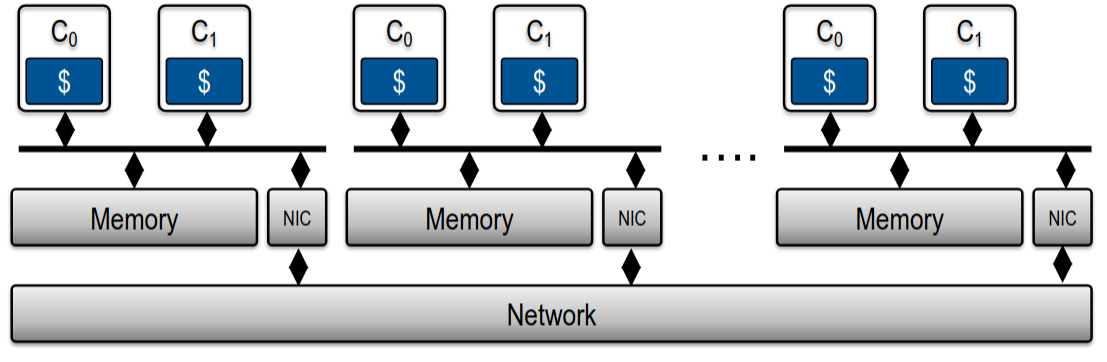
\includegraphics[width=9cm]{images/24.png}
    \end{center}
    \begin{tcolorbox}[gris]
        Advantages of message passing are:
        \begin{itemize}[left=10pt, label=\textbullet]
            \item The cost scalability: cache-coherent shared memory becomes expensive quite fast and distributed memory without cache coherence is common. 
            \item The transparency: the communication is explicit (send/receive messages).
            \item The fault tolerance: if a process fail it doesn't crash the entire system.
        \end{itemize}
    \end{tcolorbox}
    \begin{tcolorbox}[gris]
        Disadvantages of message passing are:
        \begin{itemize}[left=10pt, label=\textbullet]
            \item There is a higher communication overhead: syscalls, user-level library, etc \ldots 
            \item It increases the code complexity. 
            \item It is difficult to overlap with computation: while the message is traveling its hard to compute at the same time.
        \end{itemize}
    \end{tcolorbox}
\subsection{MPI}
    \begin{tcolorbox}[vert]
        To apply message passing we use \important{MPI (Message Passing Interface)}. The model of MPI is a \important{SPMD (Single Program Multiple Data)} model: each process has a copy of the same program and they all run at their own rate and can take different paths through the code.
    \end{tcolorbox}
    A simple code using MPI looks like this:
    \begin{codeCenter}
    \begin{Ccode}
#include "mpi.h" //include the MPI libraries
#include <stdio.h>
int main(int argc, char *argv[])
{
    MPI_Init(&argc, &argv); //Initializes MPI env.
    printf("Hello, world!\n");
    MPI_Finalize(); //End of MPI section
    return 0;
}
    \end{Ccode}
    \end{codeCenter}
    \begin{tcolorbox}[vert]
       MPI processes can be collected into groups and MPI identifies groups by their context.\\
       \important{MPI communicators} are combination of a group and its context. Groups can sometimes overlap.
    \end{tcolorbox}
    \begin{tcolorbox}[gris]
        \textbf{Some facts on communicators:}\\
        On starting an MPI program there is one predefined communicator called \lstinline!MPI_COMM_WORLD! that contains the group of all processes.\\
        A process is identified by a unique number within each communicator, its called the rank of a process, and the same process can have different rank in different communicators when groups overlap.\\
        The utility of communicators is to minimize unnecessary communications, but simple programs usually only use \lstinline!MPI_COMM_WORLD!.
    \end{tcolorbox}
    If we want to customize our ``Hello world'':
    \begin{codeCenter}
    \begin{Ccode}
#include "mpi.h"
#include <stdio.h>
int main( int argc, char *argv[] )
{
    int rank, size;
    MPI_Init( &argc, &argv );
    //Get the rank of the process
    MPI_Comm_rank(MPI_COMM_WORLD, &rank); 
    //Get the # of the process
    MPI_Comm_size(MPI_COMM_WORLD, &size); 
    printf("I am process %d of %d.\n", rank, size);
    MPI_Finalize();
    return 0;
}
    \end{Ccode}
    \end{codeCenter}
    In MPI both process must take action to communicate: one have to send and the other have to receive.

    \begin{tcolorbox}[violet]
        
        \textbf{Send:} \lstinline!MPI_Send! is a blocking function call, it returns when message has been delivered to the system but it doesn't imply that the message has been received by the target process. There exist variant with different effects:
        \begin{itemize}[left=10pt]
            \item \lstinline!MPI_Bsend!: it returns when the message is buffered in an application buffer (doesn't wait at all before returning), 
            \item \lstinline!MPI_Ssend!: it returns only when receiver has started to receive the message,
            \item \lstinline!MPI_Rsend!: assuming receiver is ready (is waiting), message is sent asap.
        \end{itemize}
    \end{tcolorbox}
    \begin{tcolorbox}[violet]
        \textbf{Receive:} \lstinline!MPI_Recv! is also a blocking function call, its source can be \lstinline!MPI_ANY_SOURCE! to accept data from any sender and the tag can be \lstinline!MPI_ANY_TAG! to accept messages with any tag. The status contains further information but we can ignore with \lstinline!MPI_STATUS_IGNORE!.
    \end{tcolorbox}
    \textbf{Communicating arrays:}\\
    There is different approach to send arrays with MPI, the first one would be to send elements one by one, or to send the entire array at once.
    \begin{codeCenter}
    \begin{Ccode}
int A[1000];
for(int i = 0; i < 1000; i++) {
    MPI_Send(&A[i], 1, MPI_INT, rank, tag, MPI_COMM_WORLD);
}
    \end{Ccode}
    \end{codeCenter}
    Or, 
    \begin{codeCenter}
    \begin{Ccode}
int A[1000];
MPI_Send(A, 1000, MPI_INT, rank, tag, MPI_COMM_WORLD);
    \end{Ccode}
    \end{codeCenter}
    A hybrid approach is often the best (chunks of 100 elements), the first approach creates too much overhead and the second one solicit the memory and spam the cache if arrays are too big.
    
    For short messages, latency dominates transfer time, but for long messages this is bandwidth. 
    \begin{tcolorbox}[vert]
        The \important{critical message size} is the amount of buffer that exists in the system, you can find it by computing 
        \[\text{latency} \cdot  \text{bandwidth}.\]
    \end{tcolorbox}
    \begin{tcolorbox}[rouge]
        \textbf{Ping-pong between two processes example:}
\begin{codeCenter}
\begin{Ccode}
int ping_pong_count = 0;
int partner_rank = (rank + 1) % 2;
while (ping_pong_count < PING_PONG_LIMIT) {
    if (rank == ping_pong_count % 2) {
        // Increment the ping pong count before you send it
        ping_pong_count++;
        MPI_Send(&ping_pong_count, 1, MPI_INT, partner_rank, 0, MPI_COMM_WORLD);
        printf("%d sent and incremented %d to %d\n", rank,ping_pong_count, partner_rank);
    } else {
        MPI_Recv(&ping_pong_count, 1, MPI_INT, partner_rank, 0, MPI_COMM_WORLD,MPI_STATUS_IGNORE);
        printf("%d received %d from %d\n", rank, ping_pong_count,partner_rank);
    }
}
\end{Ccode}
\end{codeCenter}
    \end{tcolorbox}
    \newpage 
    MPI functions are blocking functions, it means that sometimes deadlocks can occurs if the code isn't written correctly.
    \begin{image}{For example, in this code, the process 0 is stuck sending data, and process 1 is also stuck sending data. Neither can invoke \lstinline!MPI_Recv! to the data.}
        \begin{codeCenter}
        \begin{Ccode}
if(rank == 0){
    MPI_Send(...);
    MPI_Recv(...);
} else if(rank == 1){
    MPI_Send(...);
    MPI_Recv(...);
}
        \end{Ccode}
        \end{codeCenter}
    \end{image}
    \begin{image}{Here, to fix this problem if order is known, we simply have to order functions correctly.}
        \begin{codeCenter}
        \begin{Ccode}
if(rank == 0){
    MPI_Send(...);
    MPI_Recv(...);
} else if(rank == 1){
    MPI_Recv(...);
    MPI_Send(...);
}
        \end{Ccode}
        \end{codeCenter}
    \end{image}
    Due to blocking, we also have performance blocking:
    \begin{center}
    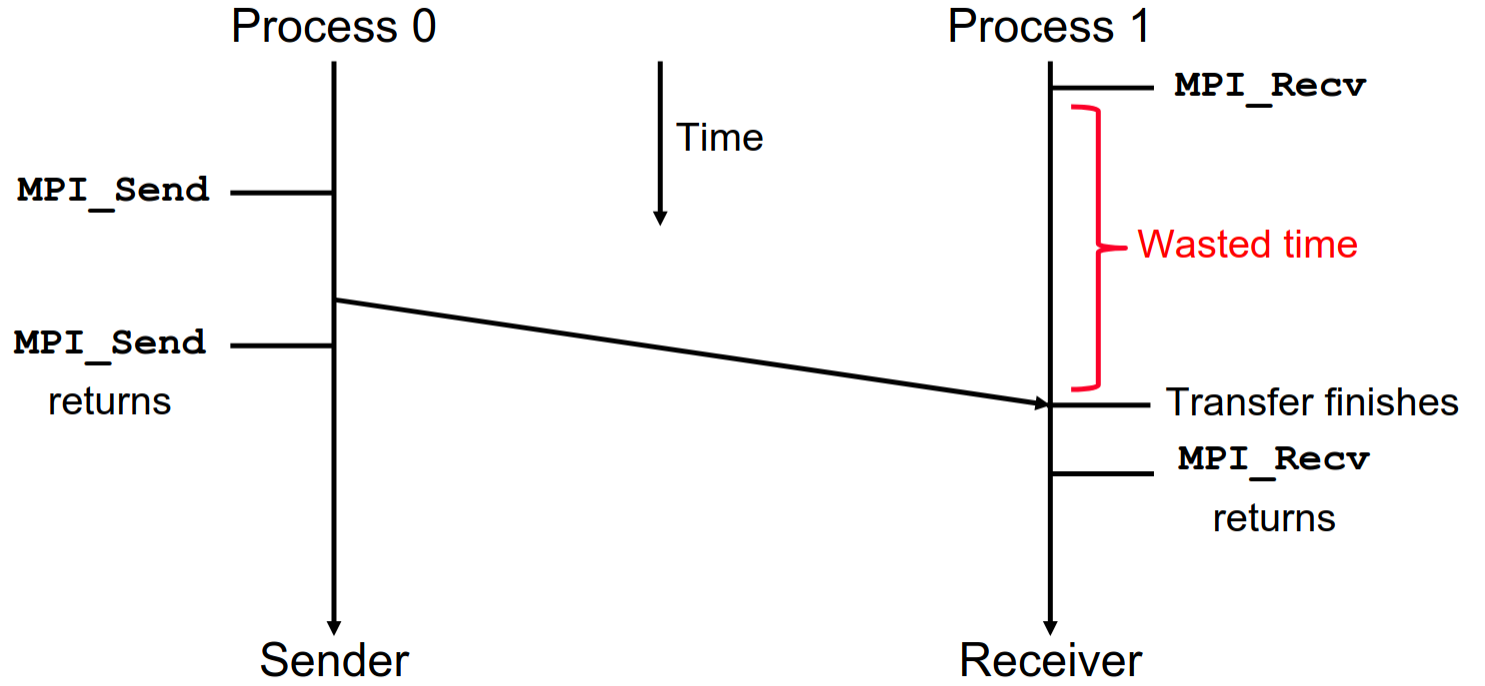
\includegraphics[width=9cm]{images/25.png}
    \end{center}
    \begin{tcolorbox}[vert]
        To avoid this we can use \important{asynchronous communication}.
        Non-blocking function calls return immediately after invocation but they doesn't provide any guarantee on the status of the message, so the programmer have to check manually for completion of message transfer. It requires more programmer effort but allows to overlap communication with computation and increase the efficiency and performance of the program.
    \end{tcolorbox}
    \begin{image}{Asynchronous transfer can be used in this situation. Process does not wait before moving on to different data.}
        \begin{codeCenter}
        \begin{Ccode}
*buf1 = 3;
MPI_Isend(buf1, 1, MPI_INT,.. 
*buf2 = 4;
        \end{Ccode}
        \end{codeCenter}
    \end{image}
    \begin{image}{But in this situation it's not possible. This is non-deterministinc, receiver can get either 3 or 4.}
        \begin{codeCenter}
        \begin{Ccode}
*buf1 = 3;
MPI_Isend(buf1, 1, MPI_INT,.. 
*buf1 = 4;
        \end{Ccode}
        \end{codeCenter}
    \end{image}
    \subsection{MPI collectives}
        Some MPI instructions: 
        \begin{itemize}[left=10pt, label=\textbullet]
            \item \textbf{Broadcast:}

                \begin{image}{It sends the same data to all processes in the group in a time $O\left(\log_2\left(n\right)\right)$.}
                    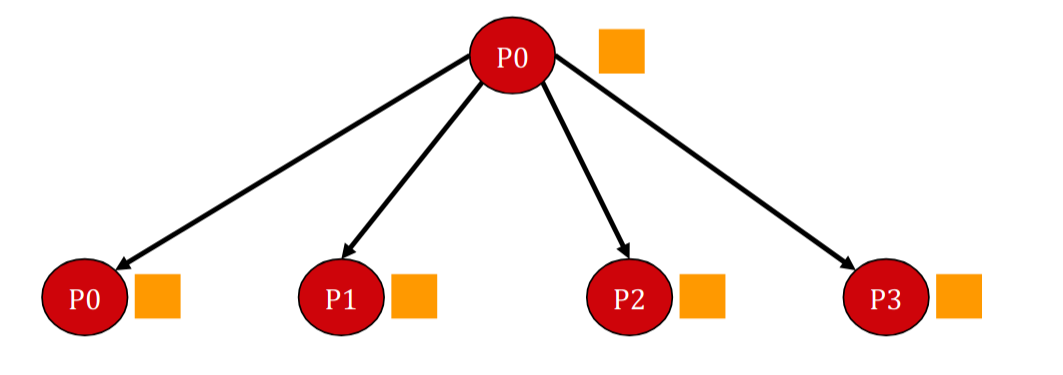
\includegraphics[width=7cm]{images/26.png}
                \end{image}
            \item \textbf{Scatter:}
                \begin{image}{It sends elements in an array to consecutive processes in a group, the data is transmitted in increasing order of process rank.}
                    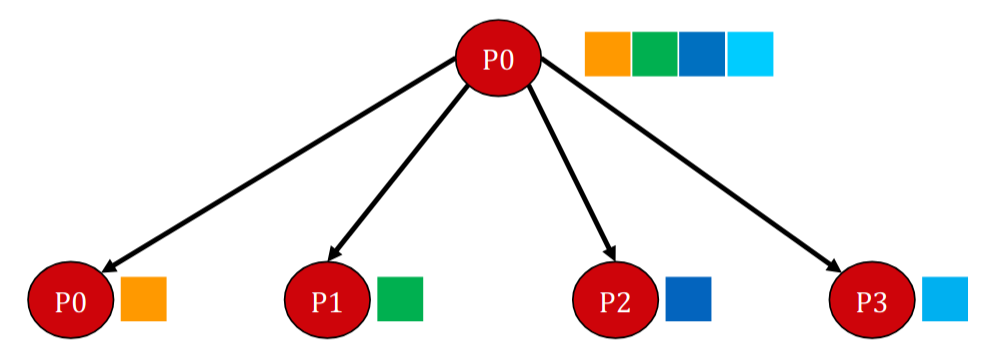
\includegraphics[width=7cm]{images/27.png}
                \end{image}
            \item \textbf{Gather:}
                \begin{image}{It gathers elements from consecutive processes in group into an array.}
                    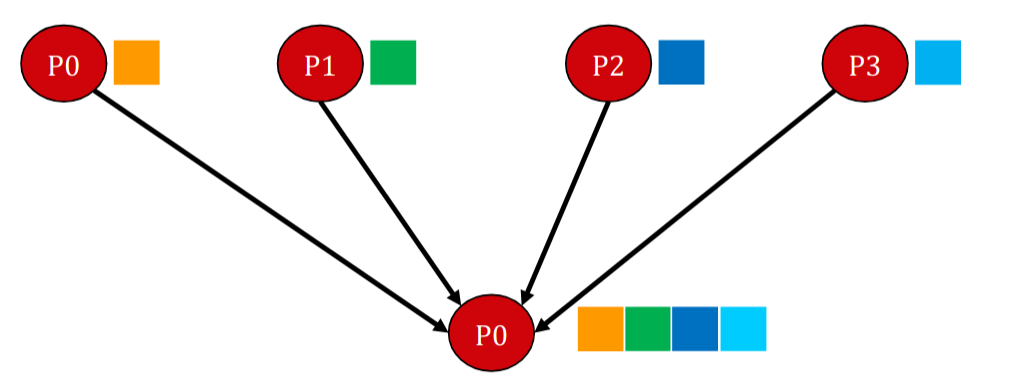
\includegraphics[width=7cm]{images/28.png}
                \end{image}
            \item \textbf{Reduce:}
                \begin{image}{It takes an array of input elements on each process and returns an array of output elements to the root process given a specific operation.}
                    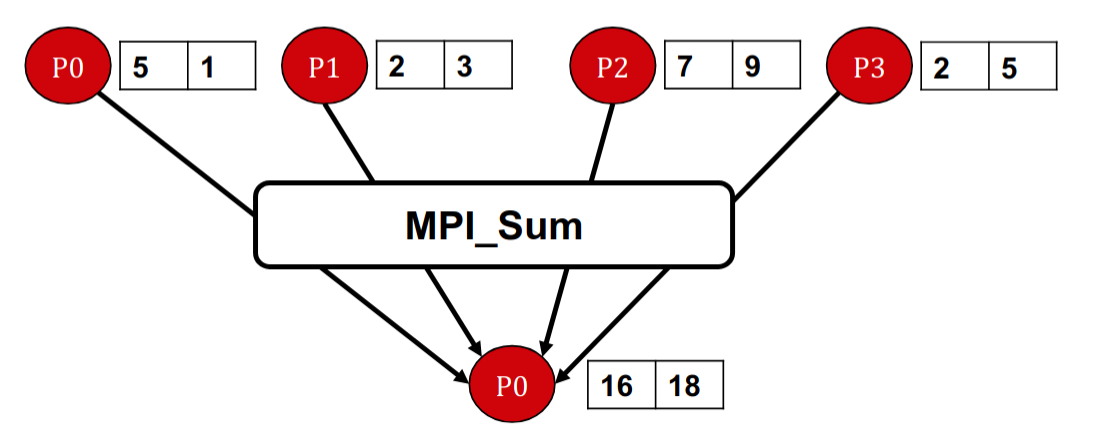
\includegraphics[width=7cm]{images/29.png}
                \end{image}
            \item \textbf{AllReduce:}
                \begin{image}{It's similar to reduce but results are distributed to all processes}
                    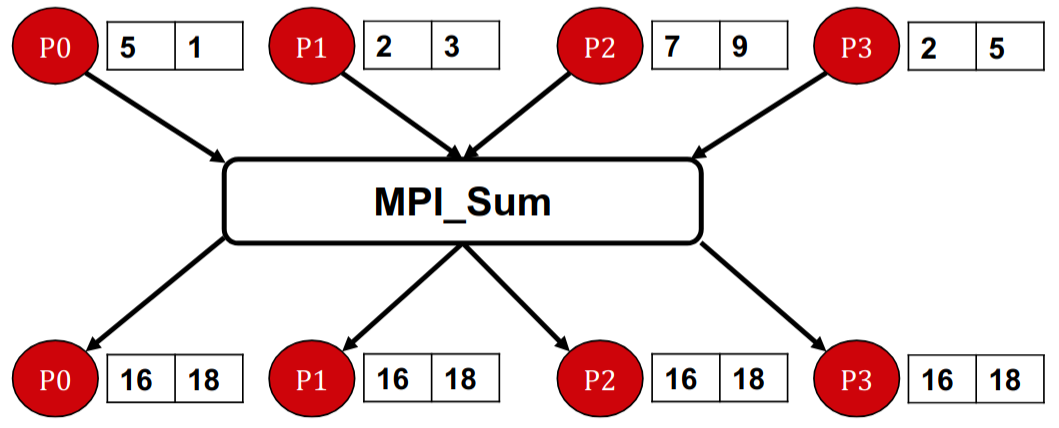
\includegraphics[width=7cm]{images/30.png}
                \end{image}
            \item \textbf{Scan:}
                \begin{image}{Similar to AllReduce but with partial results}
                    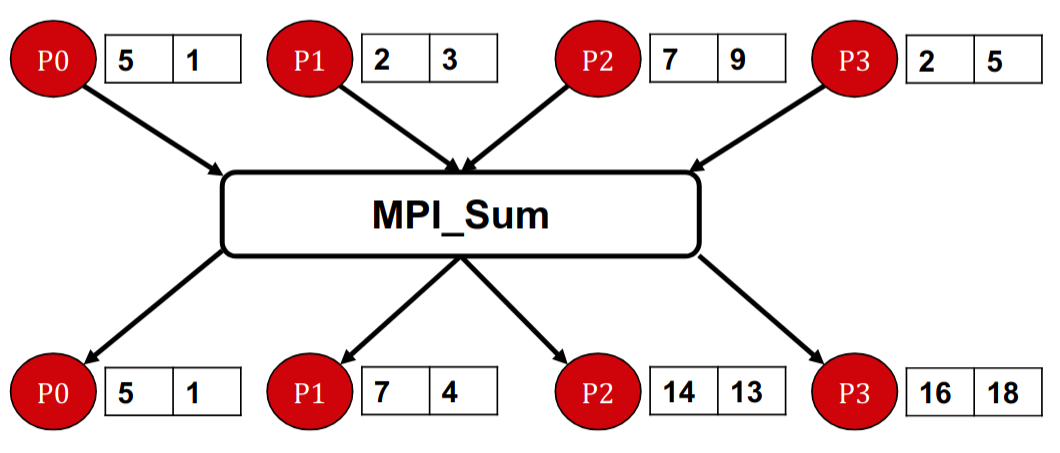
\includegraphics[width=7cm]{images/31.png}
                \end{image}
        \end{itemize}
